
%%% Local Variables: 
%%% mode: latex
%%% TeX-master: t
%%% End: 

\documentclass[11pt, letterpaper,twocolumn]{article}
%\teusepackage[utf8]{inputenc}
\usepackage[spanish]{babel}
\usepackage{lettrine}
\usepackage[top=1.5in, bottom=1.00in, left=0.85in, right=0.65in]{geometry}
\usepackage{wrapfig}
\usepackage{xltxtra}
\usepackage{xcolor}
\usepackage{titlesec}
\usepackage{listings}
\usepackage{float}
\usepackage{subfig}
\usepackage{float}
\usepackage{url}
\lstdefinestyle{customasm}{
  belowcaptionskip=1\baselineskip,
  xleftmargin=\parindent,
  language=[x86masm]Assembler,
  basicstyle=\footnotesize\ttfamily,
  commentstyle=\color{light-gray},
  basicstyle=\footnotesize\ttfamily, % Standardschrift
  numbers=left,               % Ort der Zeilennummern
  numberstyle=\tiny,          % Stil der Zeilennummern
  backgroundcolor=\color{light-gray},
  belowcaptionskip=0em,
}
\lstdefinestyle{custombash}{
  belowcaptionskip=1\baselineskip,
  basicstyle=\footnotesize\ttfamily,
  commentstyle=\color{light-gray},
  basicstyle=\footnotesize\ttfamily, % Standardschrift
  backgroundcolor=\color{light-gray},
  belowcaptionskip=0em,
}
\renewcommand*{\lstlistingname}{Código}
\definecolor{inil}{HTML}{3B9CB2}
\definecolor{titles}{HTML}{751D3E}
\setmainfont{Roboto Slab}
\definecolor{light-gray}{gray}{0.95}
%7in x 8.5in
%3.25in x 8.5in
\setlength{\columnsep}{0.5cm}

\titleformat{\section}
{\color{titles}\normalfont\LARGE\bfseries}
{\color{titles}\thesection}{1em}{}

\titleformat{\subsection}
{\color{titles}\normalfont\normalsize\bfseries}
{\color{titles}\thesubsection}{1em}{}

\newcommand{\capword}[1]{
	\lettrine[lines=3,  lraise=0.3, lhang=0.2]{\textcolor{inil}{#1}}{}
}
\floatstyle{boxed}
\restylefloat{figure}
\DeclareGraphicsExtensions{.png}
\graphicspath{{img/}}

\DeclareCaptionFont{white}{\color{white}}
\DeclareCaptionFormat{listing}{\colorbox[cmyk]{0.43, 0.35, 0.35,0.01}{\parbox{\columnwidth}{\hspace{15pt}#1#2#3}}}
\captionsetup[lstlisting]{format=listing,labelfont=white,textfont=white, singlelinecheck=true, margin=0pt, font={bf,footnotesize}}
\begin{document}
% \documentclass[11pt, letterpaper,twocolumn]{article}
% %\teusepackage[utf8]{inputenc}
% \usepackage[spanish]{babel}
% \usepackage{lettrine}
% \usepackage[top=1.5in, bottom=1.00in, left=0.85in, right=0.65in]{geometry}
% \usepackage{wrapfig}
% \usepackage{xltxtra}
% \usepackage{xcolor}
% \usepackage{titlesec}
% \usepackage{listings}
% \usepackage{float}
% \usepackage{subfig}
% \usepackage{float}
% \usepackage{url}
% \lstdefinestyle{customasm}{
%   belowcaptionskip=1\baselineskip,
%   xleftmargin=\parindent,
%   language=[x86masm]Assembler,
%   basicstyle=\footnotesize\ttfamily,
%   commentstyle=\color{light-gray},
%   basicstyle=\footnotesize\ttfamily, % Standardschrift
%   numbers=left,               % Ort der Zeilennummern
%   numberstyle=\tiny,          % Stil der Zeilennummern
%   backgroundcolor=\color{light-gray},
%   belowcaptionskip=0em,
% }
% \renewcommand*{\lstlistingname}{Código}
% \definecolor{inil}{HTML}{3B9CB2}
% \definecolor{titles}{HTML}{751D3E}
% \setmainfont{Roboto Slab}
% \definecolor{light-gray}{gray}{0.95}
% %7in x 8.5in
% %3.25in x 8.5in
% \setlength{\columnsep}{0.5cm}

% \titleformat{\section}
% {\color{titles}\normalfont\LARGE\bfseries}
% {\color{titles}\thesection}{1em}{}

% \titleformat{\subsection}
% {\color{titles}\normalfont\normalsize\bfseries}
% {\color{titles}\thesubsection}{1em}{}

% \newcommand{\capword}[1]{
% 	\lettrine[lines=3,  lraise=0.3, lhang=0.2]{\textcolor{inil}{#1}}{}
% }
% \floatstyle{boxed}
% \restylefloat{figure}
% \DeclareGraphicsExtensions{.png}
% \graphicspath{{img/}}

% \DeclareCaptionFont{white}{\color{white}}
% \DeclareCaptionFormat{listing}{\colorbox[cmyk]{0.43, 0.35, 0.35,0.01}{\parbox{\columnwidth}{\hspace{15pt}#1#2#3}}}
% \captionsetup[lstlisting]{format=listing,labelfont=white,textfont=white, singlelinecheck=true, margin=0pt, font={bf,footnotesize}}
% \begin{document}
\section{Introducción}

\capword{En} la actualidad, las computadoras y dispositivos electrónicos nos
rodean. Desde las clásicas computadoras hasta televisiones con
microprocesadores incluidos. Todos estos dispositivos requieren de herramientas
de software para facilitar su uso y desarrollo de aplicaciones. Los sistemas
operativos proporcionan las herramientas mas básicas de software para estas
tareas. Existen diferentes sistemas operativos que varían en su utilidad,
herramientas o arquitectura. Estos sistemas operativos son una parte esencial
para la computación. Sin estos, los avances en computación no hubieran sido
posibles.  La pregunta por contestar es cómo se define a un sistema
operativo. De acuerdo con Andrew S. Tannenbaum en su libro \emph{Sistemas
Operativos Modernos}: ``Es difícil puntualizar que es un sistema
operativo''. Sin embargo, podemos decir que un sistema operativo contiene
herramientas esenciales orientadas a facilitar la comunicación entre el
hardware y el usuario. Cabe mencionar que los usuarios a los que haremos
referencia y a los que están orientados estas herramientas es principalmente a
desarrolladores y usuarios avanzados o \emph{power users}. En adelante, la
discusión del desarrollo de sistemas operativos se centrará en la manera de
implementar estos servicios básicos, dejando de lado temas como el ambiente de
ventanas o interfaces dirigidas al consumidor común.

\subsection{Computer Architecture Overview}

Para poder diseñar y por consecuencia entender como funcionan los sistemas
operativos, es necesario entender el concepto detrás de las funcionalidades de
los microprocesadores actuales. El poder entender el concepto abstracto detras
de la concepción de las computadoras es esencial para entender la manera en que
estas fueron diseñadas y por consecuencia las necesidades que debe cubrir un
sistema operativo.

Todos los dispositivos actuales que hacen uso de microprocesadores están
basados en una construcción matemática. Alan Turin definió en 1936 lo que
llegaría a conocerse como Máquina de Turing (MT).  Una MT consiste en una cinta
con símbolos, una cabeza lectora y una \emph{máquina de estados}. En la figura
\ref{fig:tm} se muestra un diagrama de una MT. 

\begin{figure}[htbp]
  \centering
  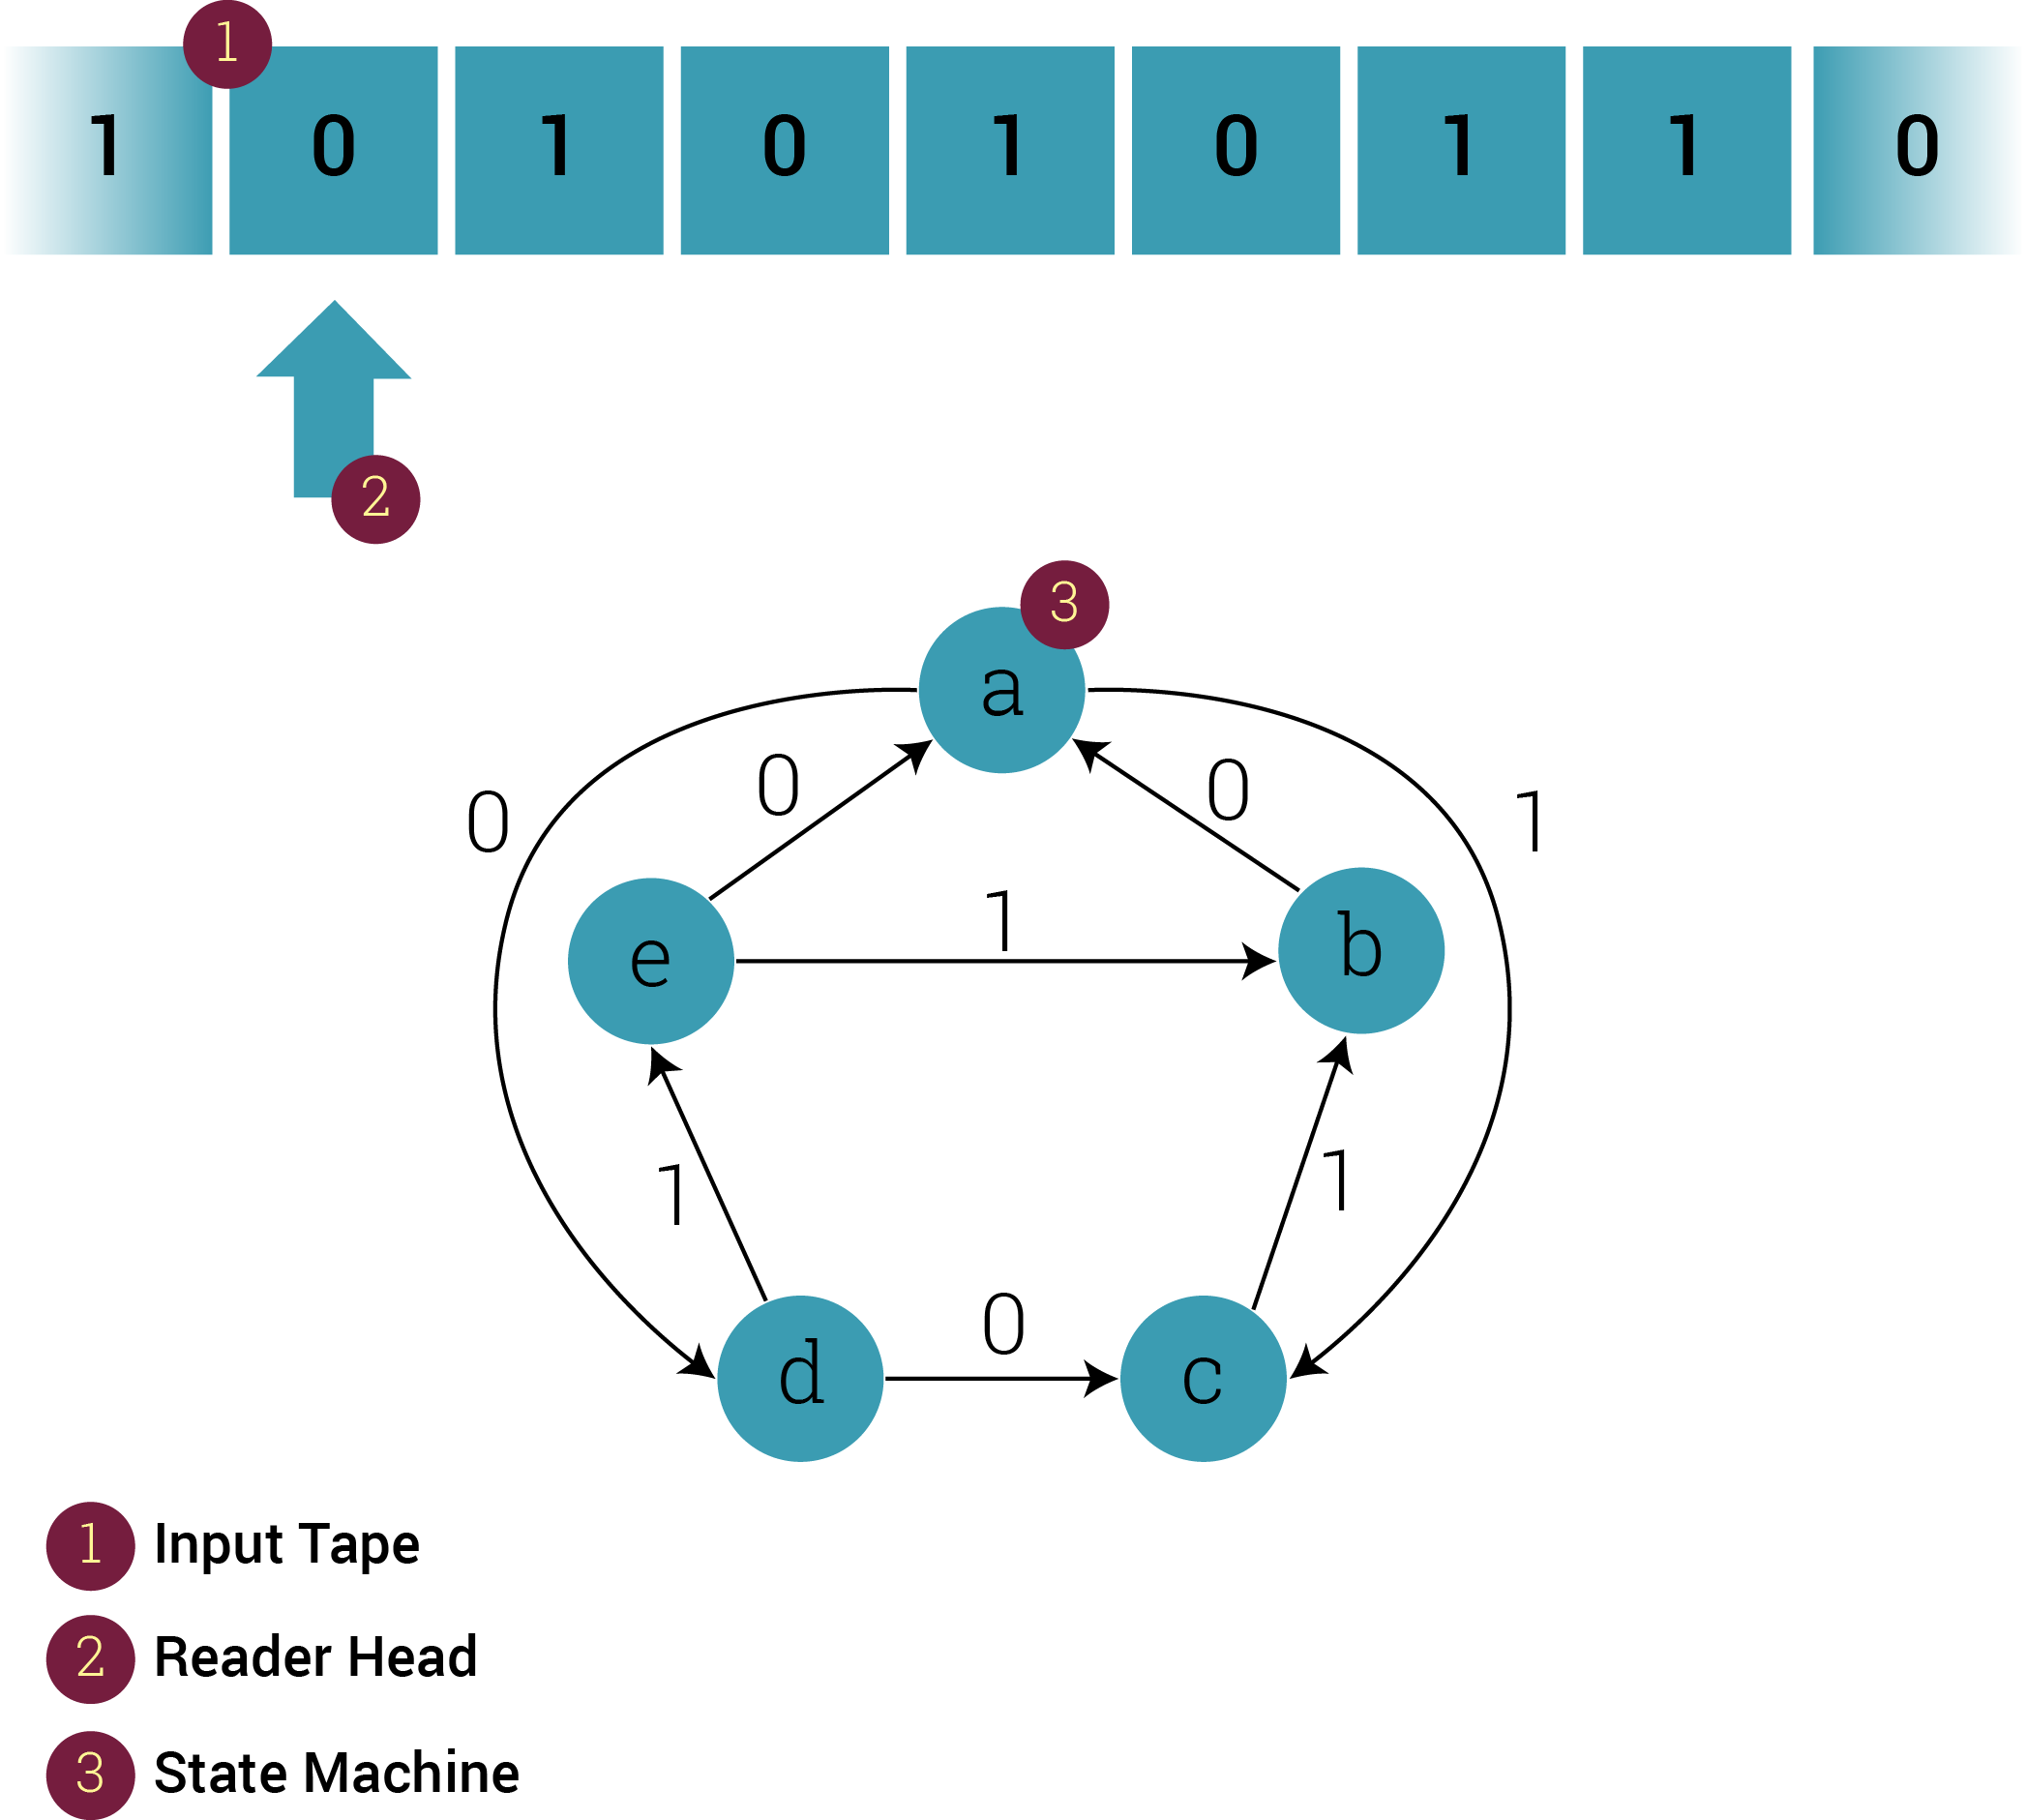
\includegraphics[width=\columnwidth]{tm}
  \caption{Representación Gráfica de una Turing Machine}
  \label{fig:tm}
\end{figure}

La operación de una MT es como sigue: La cabeza lectora avanza un lugar, lee un
símbolo de la cinta y la máquina de estados cambia su estado actual según el
símbolo leído.  Los microprocesadores modernos siguen el mismo principio. La
memoria de acceso aleatorio (RAM por sus siglas en inglés) toma el lugar de la
cinta, la cabeza lectora es un elemento del procesador conocido como
\emph{program counter} (PC) y por último la máquina de estados es el conjunto
de elementos del procesador llamados registros, como \texttt{AX} o \texttt{DS}.

\subsection{Tasks of an Operating System}

Las tareas específicas de un sistema operativo dependen en su mayoría del
objetivo con el que fue construido y el hardware donde es implementado. Sin
embargo, podemos generalizar sus tareas en dos elementos principales:

\begin{enumerate}
\item Proveer de herramientas y programas a desarrolladores y usuarios que sean
sencillas y transparentes a diferencia de lo que seria operar el hardware de
manera directa.
\item Administrar los diferentes elementos de hardware.
\end{enumerate}

Esto significa que el sistema operativo sera empacado con un conjunto de
librerias listas para ser usadas por los desarrolladores además de mantener
servicios en ejecución durante el funcionamiento de la computadora en espera de
brindar los servicios requeridos al usuario. Estos servicios son usados tanto
por desarrolladores como por usuarios comerciales, sin embargo, estos últimos
solo los usan de manera indirecta a través de herramientas más sofisticadas.
Un sistema operativo actúa como una capa intermedia entre el hardware y los
desarrolladores y usuarios para presentar una interfaz limpia, sencilla y
ordenada de lo que de otra forma sería un trabajo solo reservado para personas
entrenadas como lo era en periodos previos a la revolución de los sistemas
operativos.  Existe sistemas operativos para diferentes tareas. Desde sistemas
operativos para los main frame que ocupan cuartos enteros hasta sistemas
operativos para dispositivos móviles. Pasando por computadoras personales,
clusters, computadoras multi núcleo y multi procesador, servidores, etc.  La
maquinaria industrial también requiere de sistemas operativos especializados
como aquellos utilizados para operar conjuntos de sensores en fábricas o
sistemas de tiempo real como los que operan los aviones Boeing.

Específicamente, podemos hablar de tres elementos básicos en las tareas de un
sistema operativo: administración de la memoria, administración del tiempo de
procesador y el sistema de mensajes o IPC por las siglas del nombre en inglés
\emph{Inter-process Comunication}. 

El sistema de administración de memoria se encarga de controlar el acceso y
otorgar espacios de memoria a los procesos en ejecución solicitantes. El
sistema de administración de tiempo o scheduling se encarga de vigilar y
otorgar el uso del procesador a los diferentes procesos que se encuentren en la
cola de ejecución. Por último, el IPC es un sistema de mensajes para la
comunicación entre procesos, es decir, gracias aeste servicio, los procesos en
ejecución pueden comunicarse entre sí. Cabe destacar que no hay que confundir
el IPC con el sistema de entrada salida (\emph{I/O}). El sistema de I/O también
es un servicio otorgado por el sistema operativo pero es una comunicación
realizada en un nivel de abstracción más alto que el IPC.

\subsection{Operating System Architecture} Uno de los elementos mas importantes
y discutidos en la construccción de un sistema operativo es el kernel. La mayor
parte de la lliteratura para el diseño de los sistemas operativos se centra en
algoritmos y propuestas de diseño para el desarrollo de kernels. Otros
servicios que también son implementados en los sistemas operativos empacados
para el usuario final han sido catalogados en problemas separados al de la
implementación de un sistema operativo.

El kernel o núcleo de un sistema operativo incorpora todas las funciones de
bajo nivel requeridas para otorgar al usuario un ambiente con el que pueda
empezar a operar. Note que el objetivo del kernel es otorgar funciones para la
administracion de los recursos de hardware y no el de crear un ambiente
completo de trabajo como es el caso de los gestores de ventanas.

Actualmente existen cuatro tipos de diseños enfocados al kernel de un sistema
operativo: Monolithic Kernel, Microkernel, Nanokernel y Exokernel. Antes de
continuar con la descripción de cada kernel, es necesario introducir El
concepto de \emph{Ring}. Ring es un concepto de seguridad en el que se definen
capas de seguridad o anillos como se muestra en la figura \ref{fig:ring}.

\begin{figure}[htbp]
  \centering
  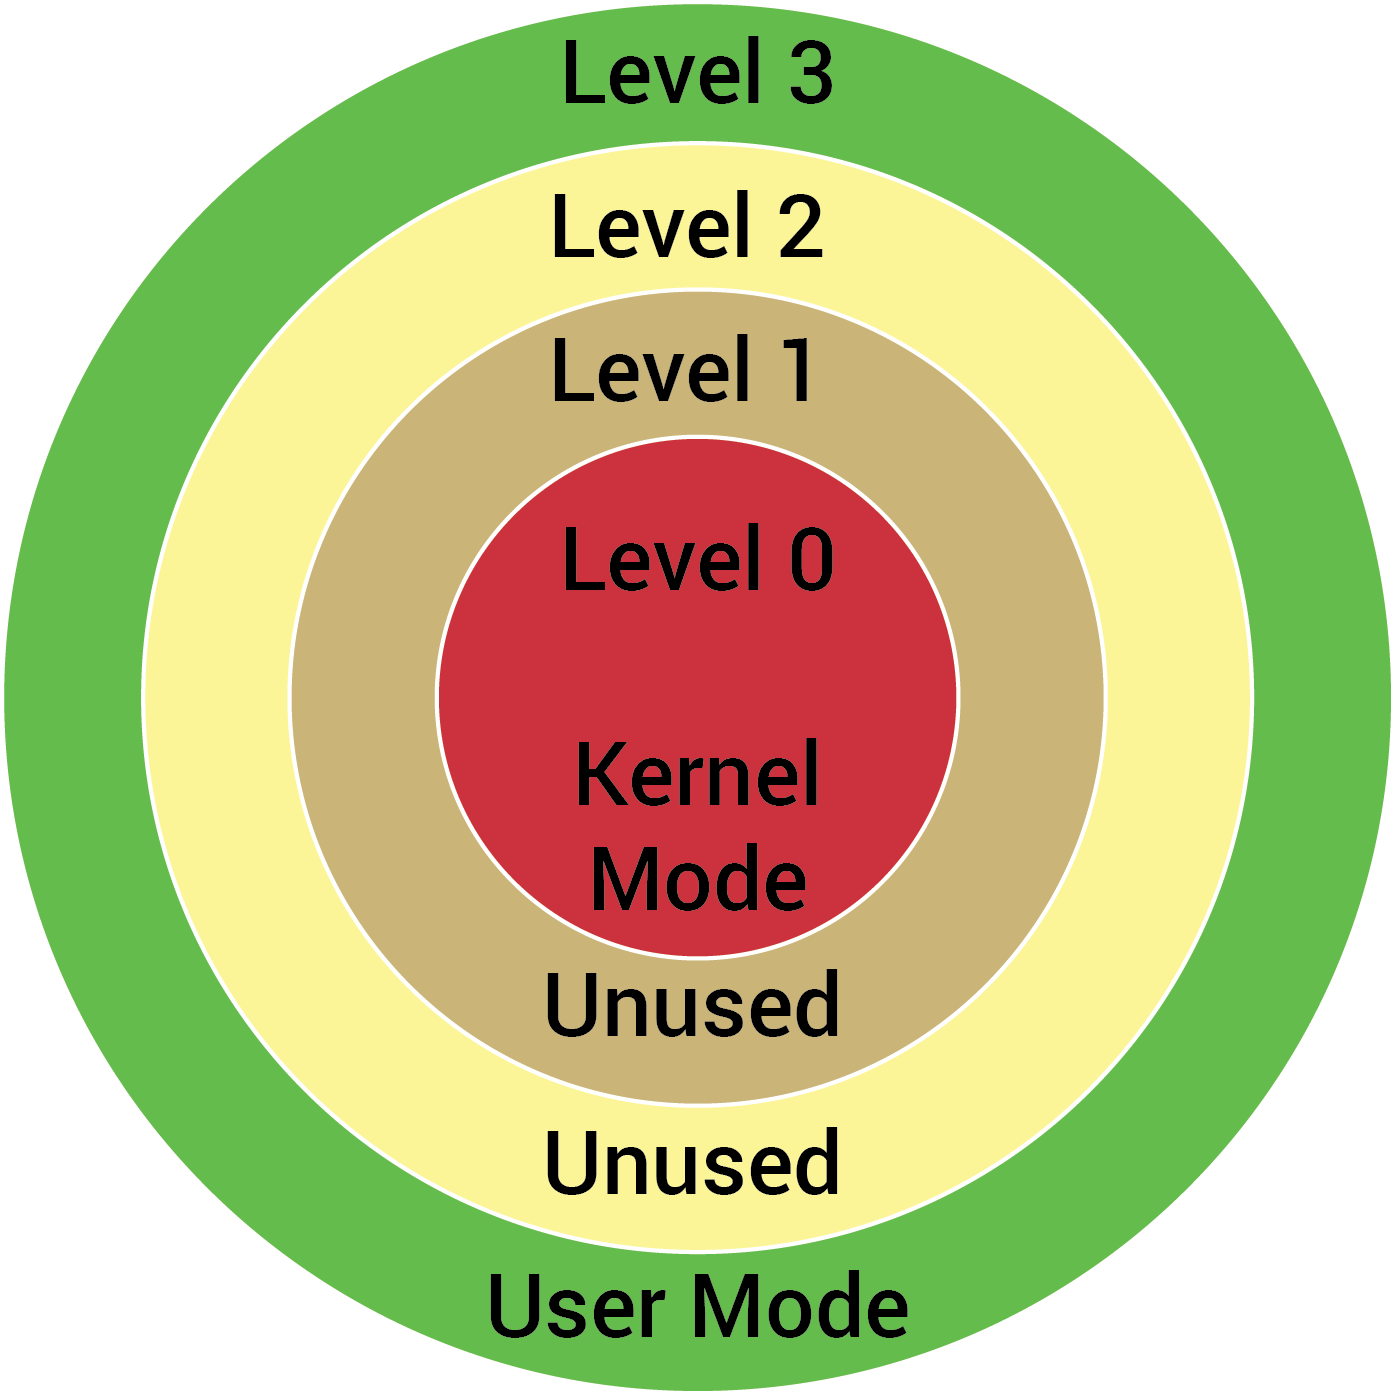
\includegraphics[width=\columnwidth]{ring}
  \caption{Anillos de Seguridad en al Arquitectura x86}
  \label{fig:ring}
\end{figure}

Los servicios de un sistema operativo son ejecutados dentro de un anillo
específico y no tiene acceso a modificar los servicios de capas inferiores de
manera arbitraria. Este esquema de seguridad es soportado a nivel de
hardware. En particular, las memorias comerciales para computadoras personales
soportan dos anillos. A estos dos anillos se les conoce como \emph{kernel mode}
y \emph{user mode}. La intención del \emph{kernel mode} también conocido como
\emph{nivel 0} es la de ejecutar todos los servicios críticos del kernel dentro
de este nivel, manteniendo los servicios del usuario dentro del \emph{user
mode} o \emph{nivel 3}. Esto evita que un usuario tenga acceso al hardware de
manera directa o modifique el estado de un servicio inadvertidamente, o
intencionalmente en el caso de virus de computadora o usuarios maliciosos. Otra
de las razones de porque usar estos dos niveles a nivel de hardware es para
implementar el concepto de multiusuario. En un sistema multiusuariolos usuarios
comparten recursos de hardware. Si un usuario puede hacerse con el control de
uno de estos recursos el sistema operativo se vería impedido de administrarlo y
compartirlo con otros usuarios conectados al sistema. Todos los servicios
considerados críticos se ejecutan en kernel mode. Cuales de los servicios son
críticos varía de acuerdo al tipo de arquitectura. A continuación se enumeran
los distintos tipos de arquitecturas y como sus servicios son clasificados.

\begin{enumerate}
\item Monolithic Kernel - El Monolithic Kernel es quizá el mas secillo en
  concepto. Todos los servicios de bajo nivel que administran el hardware se
  encuentran contenidos en un solo módulo. Estos servicios incluyen tiempo de
  procesador, sistema de archivos, comunicaciones, manejo de memoria, etc.  En
  principio, el código fuente del kernel puede estar separado en distintas
  librerias y archivos pero una vez compilados estos archivos todo el código
  binario resultante, conocido como imagen, se carga en una zona de memoria
  específica. Todos los servicios se ejecutan en kernel mode.
\item Microkernel - El Microkernel, desarrollado como sucesor del Monolithic
  Kernel, se caracteriza por separar la mayor parte de los servicios en un
  conjunto de modulos independientes. El modulo principal contiene elementos
  básicos como el manejo de memoria, administración de de tiempo de procesador o
  \emph{scheduling} y un sistema de mensajes o IPC básico para la comunicación
  entre módulos.  Estos servicios se ejecutan en kernel mode. El resto de los
  servicios se incorporan de manera separada al momento del arranque y se
  ejecutan en user mode. Algunos de estos servicios son el sistema de archivos y
  un IPC mas robusto.
\item Nanokernel - El nanokernel no es un término completamente
  estandarizado. En principio, el enfoque del nanokernel es otorgar los
  servicios más necesarios usando solo unas cuantas lineas de código en
  comparación con las otras arquitecturas. Además, la arquitectura esta
  enfocada en la optimización de la velocidad del sistema. Una aplicación
  particular de este kernel es en los equipos de tiempo real. Debido a que el
  sistema operativo tiene que responder en tiempos perfectamente establecidos
  con la mayor precisión posible, este tipo de kernel es uno de los más adecuados.
\item Exokernel - El Exokernel es un diseño orientado hacia el desarrollo de
  aplicaciones y librerías que entran en contacto de manera mas directa con el
  hardware. En el caso de los kernels anteriores, los dispositivos de hardware
  son presentados al usuario como capas de abstracción, como es el caso del
  sistema de archivos o librerias gráficas como DirectX u OpenGL. El exokernel
  intenta mantener la interacción con el hardware lo mas directa posible sin
  perder las capacidades de administración como es el caso de MS-DOs que permitía
  ejecutar instrucciónes directamente al hardware pero no tenía servicio de
  multiusuario o multitarea. Este kernel esta siendo desarrollado por
  universidades como el MIT, su precursora, o la universidad de
  Cambridge. Actualmente ningún sistema operativo comercial tiene este tipo de
  kernel.
\end{enumerate}

En la figura \ref{fig:kernels} al final del capítulo se hace una comparativa
entre los diferentes tipos de kernels. Note que no se muestra el nanokernel,
esto es debido a que no se a definido una estructura básica para este tipo de
kernel.

\begin{figure*}[h]
  \centering
  \subfloat[Comparativa entre el monolithic y el micro kernel]{
    \label{fig:mono-micro}
    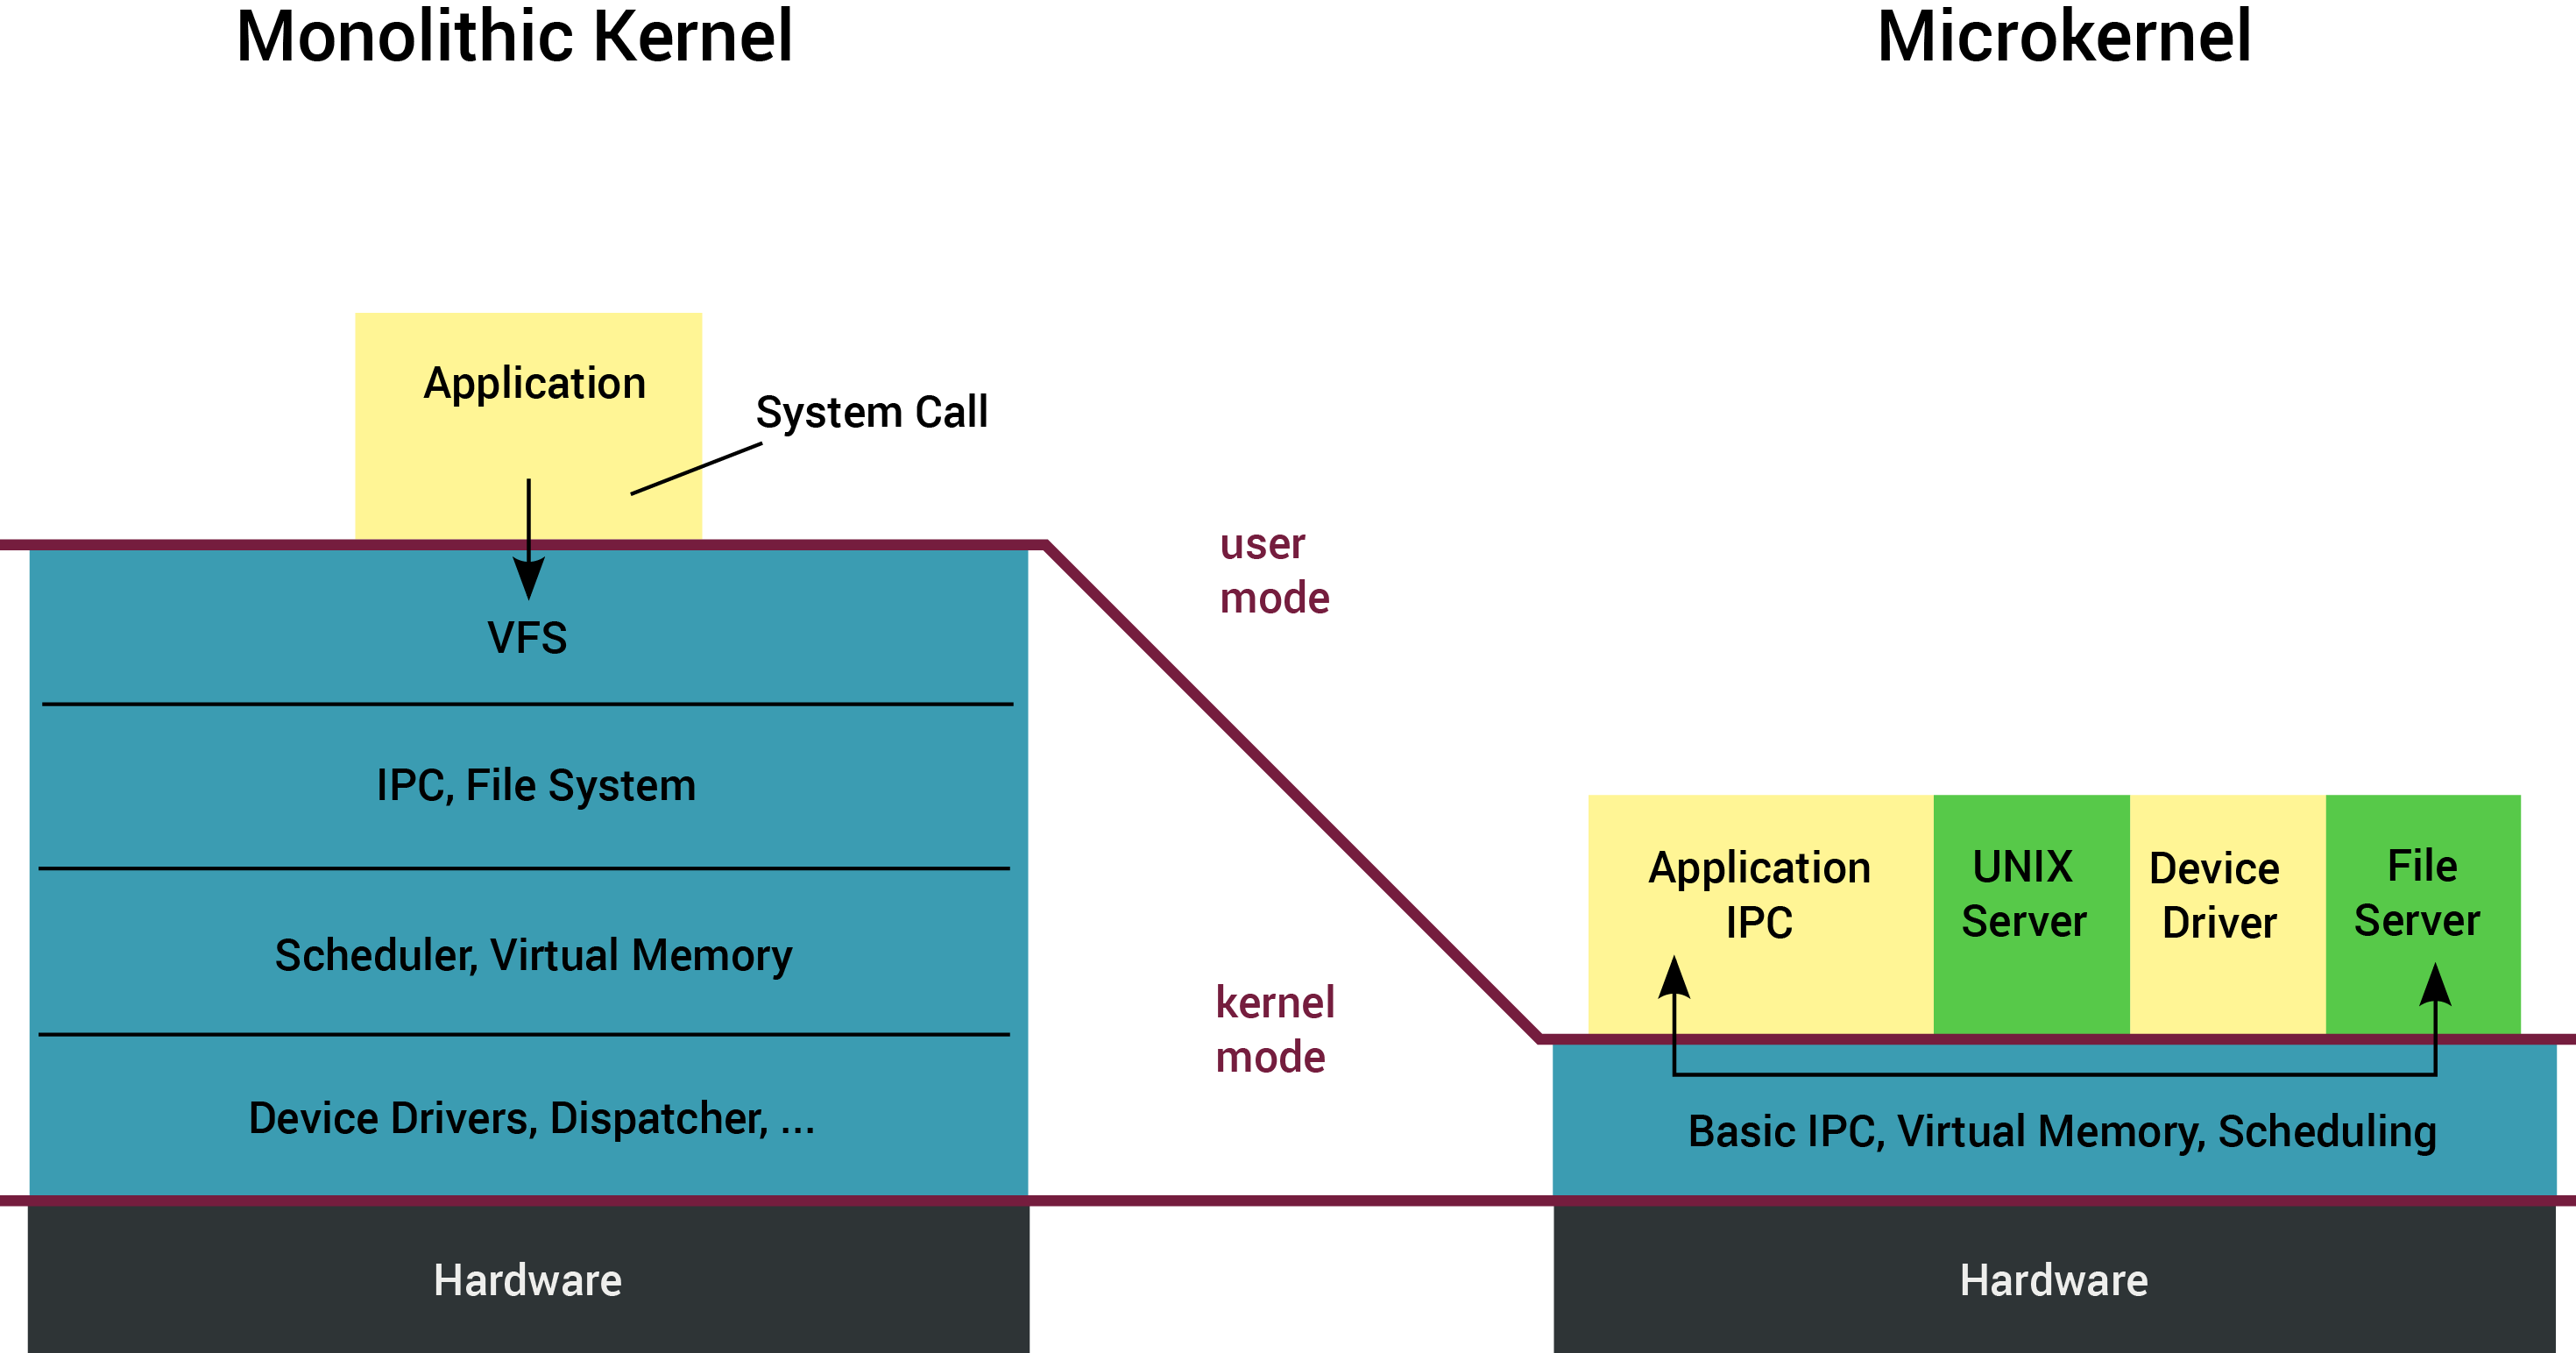
\includegraphics[width=\linewidth]{mono-micro}
  }\\
  \subfloat[Estructura del Exokernel]{
    \label{fig:exokernel}
    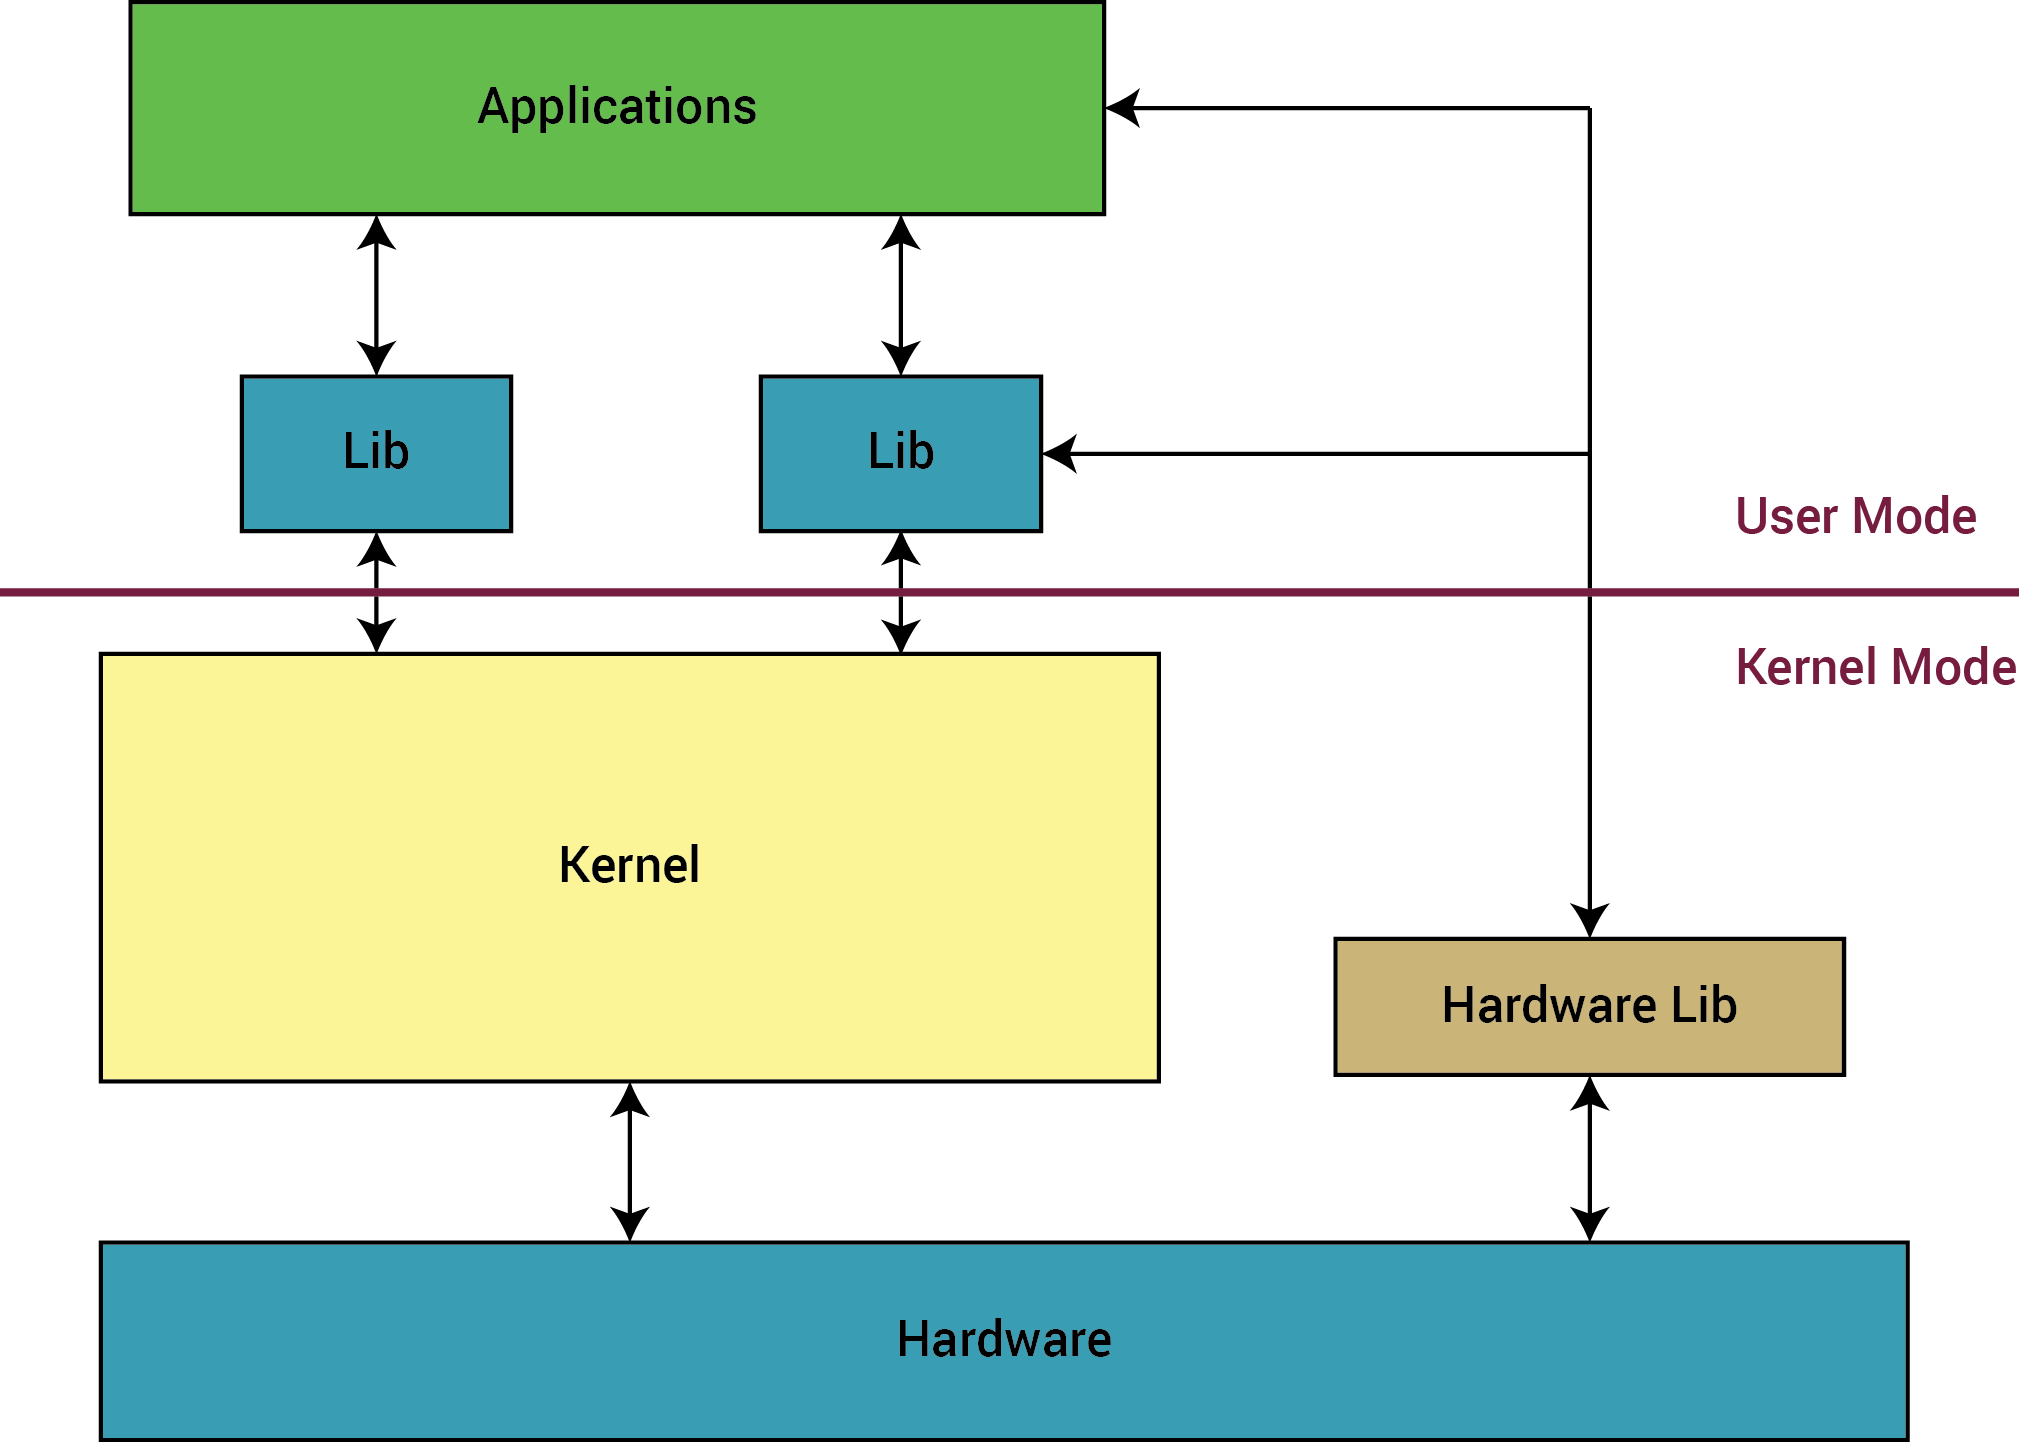
\includegraphics[width=\columnwidth]{exokernel}
  }
  \caption{Comparativa De Los Diferentes Tipos de kernel}
  \label{fig:kernels}
\end{figure*}

\subsection{Operating Systems}
En este curso se estará hablando de los tres sistemas comerciales mas populares
en las PC: Windows, Mac OS X y Linux. Además también se estudiará a sus tres
versiones móbiles: Windows Phone, Android e iOS. Sin embargo, en cuanto a los
aspectos internos solo hablaremos de Windows y Unix. Esta sección intentara
aclarar el porque.

Conocer la arquitectura básica del sistema operativo con que se trabaja permite
un mayor entendimiento de los resultados en rendimiento, velocidad y posibles
errores en los desarrollos de apliciónes, asi como también permite desarrollar
software mas fuertemente acoplado al sistema operativo como es el caso de los
drivers. En primer lugar, hay que notar que los sistemas operativos para
dispositivos móviles actuales no solo decienden de las versiones para PC sin
que son estas mismas con solo algunas modificaciones. Por esto, se revisarán
las diferentes arquitecturas que cada sistema operativo propone emparejando al
mismo tiempo la versión PC y la versión móvil.

\subsubsection{Windows} Los sistemas operativos windows han pasado por
diferentes etapas de desarrollo, empezando por su version que operaba encima de
MS-DOS desde Windows 1 hasta Windows 3.11. Después, usando la misma
arquitectura se fucionaron los dos conceptos dando como resultado las versiones
Windows 95, 98 y Me. Estas versiones estaban orientadas a usuarios
domésticos. De manera paralela, Microsoft desarrollo un sistema para servidores
con un kernel que sigue los objetivos de Unix como multi usuario y multi
tarea. Este es el kernel de las versiones NT de Windows. Windows NT es un
hybrid kernel que combina conceptos del monolithic y el micro kernel con
funciones como multitasking. Las diferentes versiones de Windows para usuarios
domésticos soportaban funciones parecidas pero el kernel no fue desarrollado en
un principio con estas características, lo que daba como resultado un
rendimiento mas pobre y algunos posibles errores. A partir de las version XP,
se decidió por fusionar los desarrollos, dejando al kernel NT como la base de
todas las versiones posteriores y limitando la compatibilidad de aplicaciones
para versiones previas del sistema operativo. A partir de Windows XP y Windows
2000, la diferencia entre versiones radica en las aplicaciones incluídas
mientras que la arquitectura base es la misma.

La arquitectura base del kernel NT se muestra en la figura \ref{fig:nt-kernel}.

\begin{figure}[H]
  \centering
  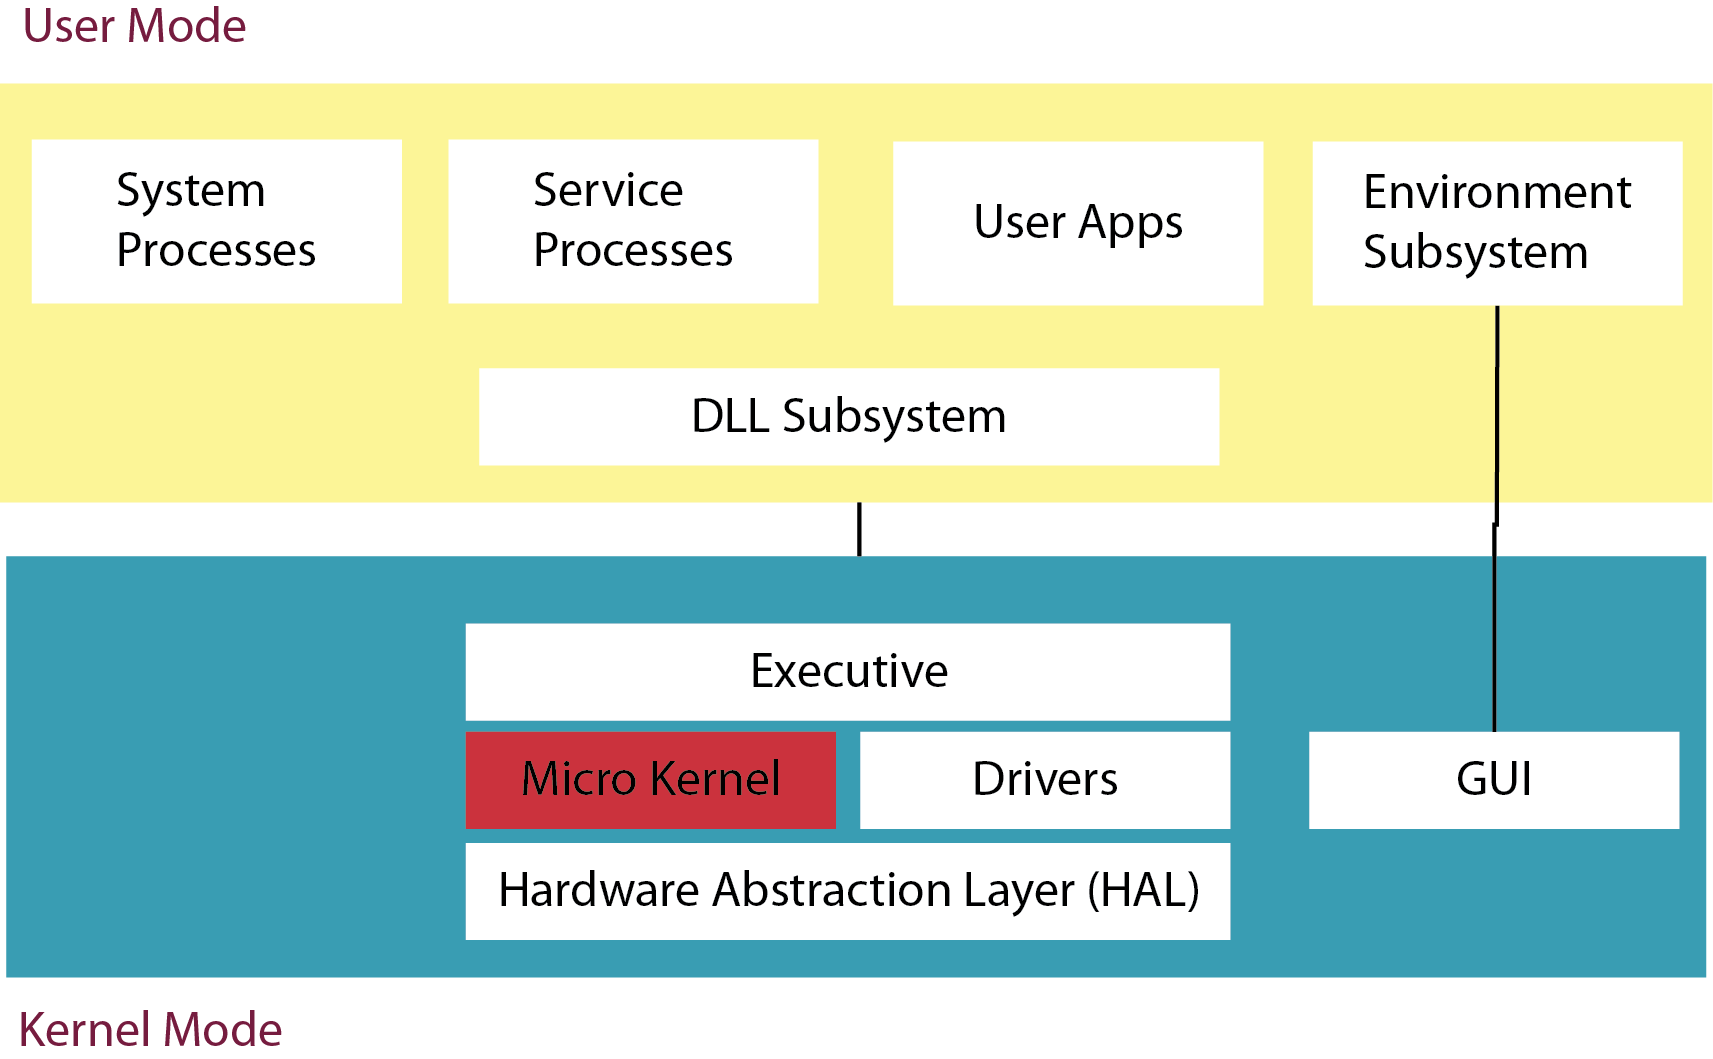
\includegraphics[width=\columnwidth]{windowsnt-arch}
  \caption{Diagrama del kernel Windows NT}
  \label{fig:nt-kernel}
\end{figure}


Para sus versiones móviles, Windows tuvo tambiém un desarrollo paralelo. Esto
debido en parte a que la arquitectura de lo dipositivos móviles era diferente y
no había un estandar claro. Los nombres de estas versiones fueron Windows
Mobile Phone y Windows CE. Con el surgimiento de ARM como estandar para estos
dispositivos, Microsoft decidió consolidar desarrollos al fusionar nuevamente
sus dos productos. El kernel resultante se implementó en Windows 7 y Windows 8
así como la aparición de su nuevo sistema operativo Windows Phone 8. La ventaja
del nuevo kernel es que puede ser compilado tanto para ARM como para x86. La
arquitectura es muy similar, dependiendo en mayor medida de su plataforma .NET
como API para los desarrolladores de aplicaciones.

\subsubsection{Linux y Android}

El sistema operativo Unix nace en la academia como una solución para la
operación de main frames y terminales tontas que manejaban ditintas
universidades. Este desarrollo fue de iniciativa académica que mas tarde sería
imitado por empresas como AT\&T. Hasta 19, el sistema operativo Unix fue
desarrollado tanto por la industria como por la academia orientándolo a
servidores y main frames. Esto dió lugar al nacimiento de diferentes versiones
de Unix como AIX y Novell. Aunque este sistema operativo podía compilarse para
arquitecturas x86, carecía de soporte para los diferentes dispositivos de
hardware. En 19, Linus Torvals comienza como proyecto de maestría el sistema
Linux basándose en la teoría desarrollada por Andrew Tannenbaum así como en el
kernel del sistema operativo que el mismo Tannenbaum estaba desarrollando:
Minix. En un golpe de suerte, Linus Torvals da a conocer a través de interntet
su desarrollo, lo que atrae a Richard Stallman, fundador de la fundación para
software libre GNU. Stallman estaba buscando crear un sistema operativo que
pudiera liberar su código fuente a todo aquel interesado y así liberar la
creatividad de los desarrolladores de licencias restrictivas. Gracias a
desarrolladores en todo el mundo y el apoyo de GNU y la despues formada Free
Software Foundation nace GNU/Linux o Linux. El kernel de Linux sigue el
estandar de Unix, siendo un 100\% compatible con el código fuente desarrollado
para Unix, salvo excepciones. Linux es un Monolithic Kernel a diferencia de
Minix que es un Microkernel. La structura básica se muestra en la figura
\ref{fig:linux-kernel}.

\begin{figure}[H]
  \centering
  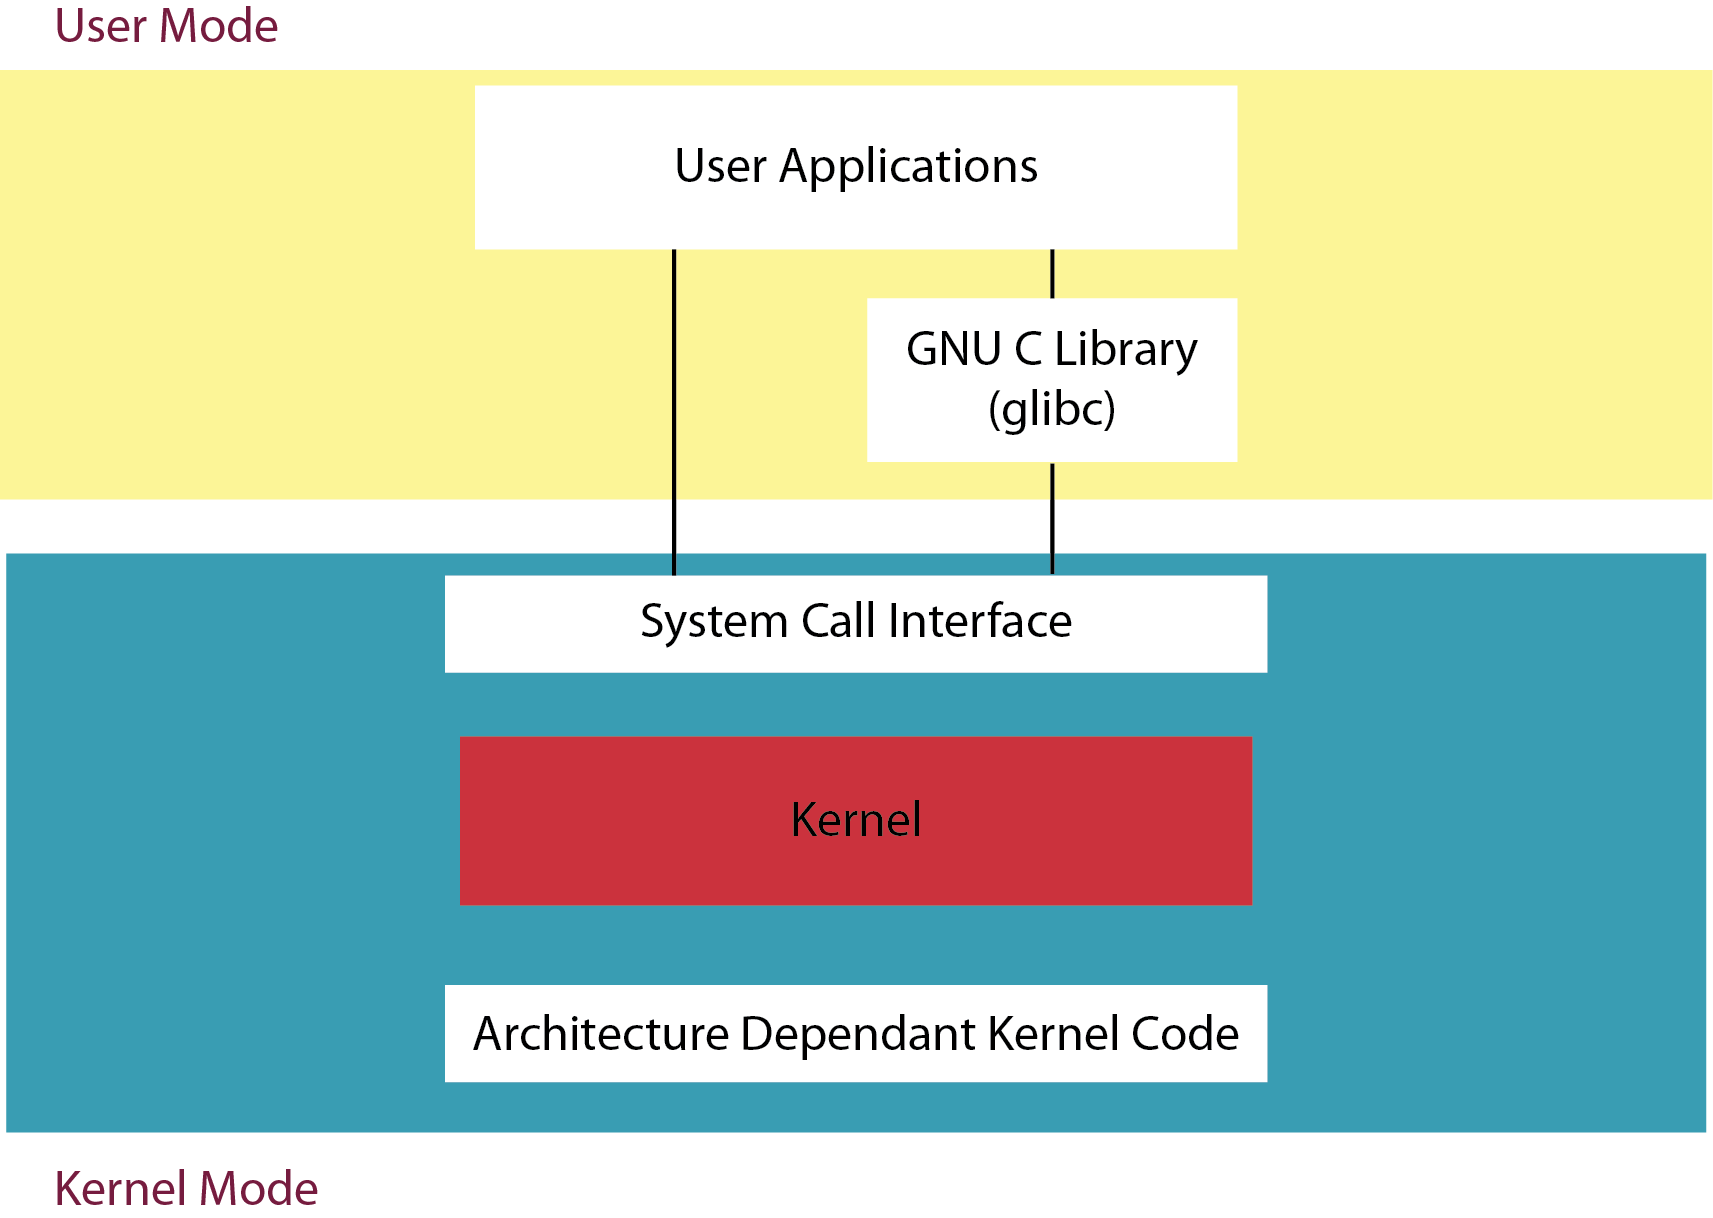
\includegraphics[width=\linewidth]{linux-arch}
  \caption{Diagrama del kernel de Linux}
  \label{fig:linux-kernel}
\end{figure}


En principio, Linux incluía el soporte a dispositivos o drivers dentro de su
kernel. Esto obligaba a recompilar el kernel de un sistema ya implementado si
se requería de agregar un dispositivo nuevo. En la actualidad se le ha dotado
con un sistema más modular que permite agregar nuevos dispositivos sin tener
que recompilar. Aún así el kernel sigue siendo tipo monolithic.

Android es un desarrollo hermano o Fork del kernel de Linux por parte de
Google. Ya que una de las ventajas de Linux es que su código es en su mayoría
portable a otras arquitecturas, ha sido la elección de muchas empresas para
crear sistemas operativos móviles. En la actualidad Android de Google ha sido
el que a prevalecido. Su arquitectura básica se muestra en la figura
\ref{fig:android-kernel}.

\begin{figure}[H]
  \centering
  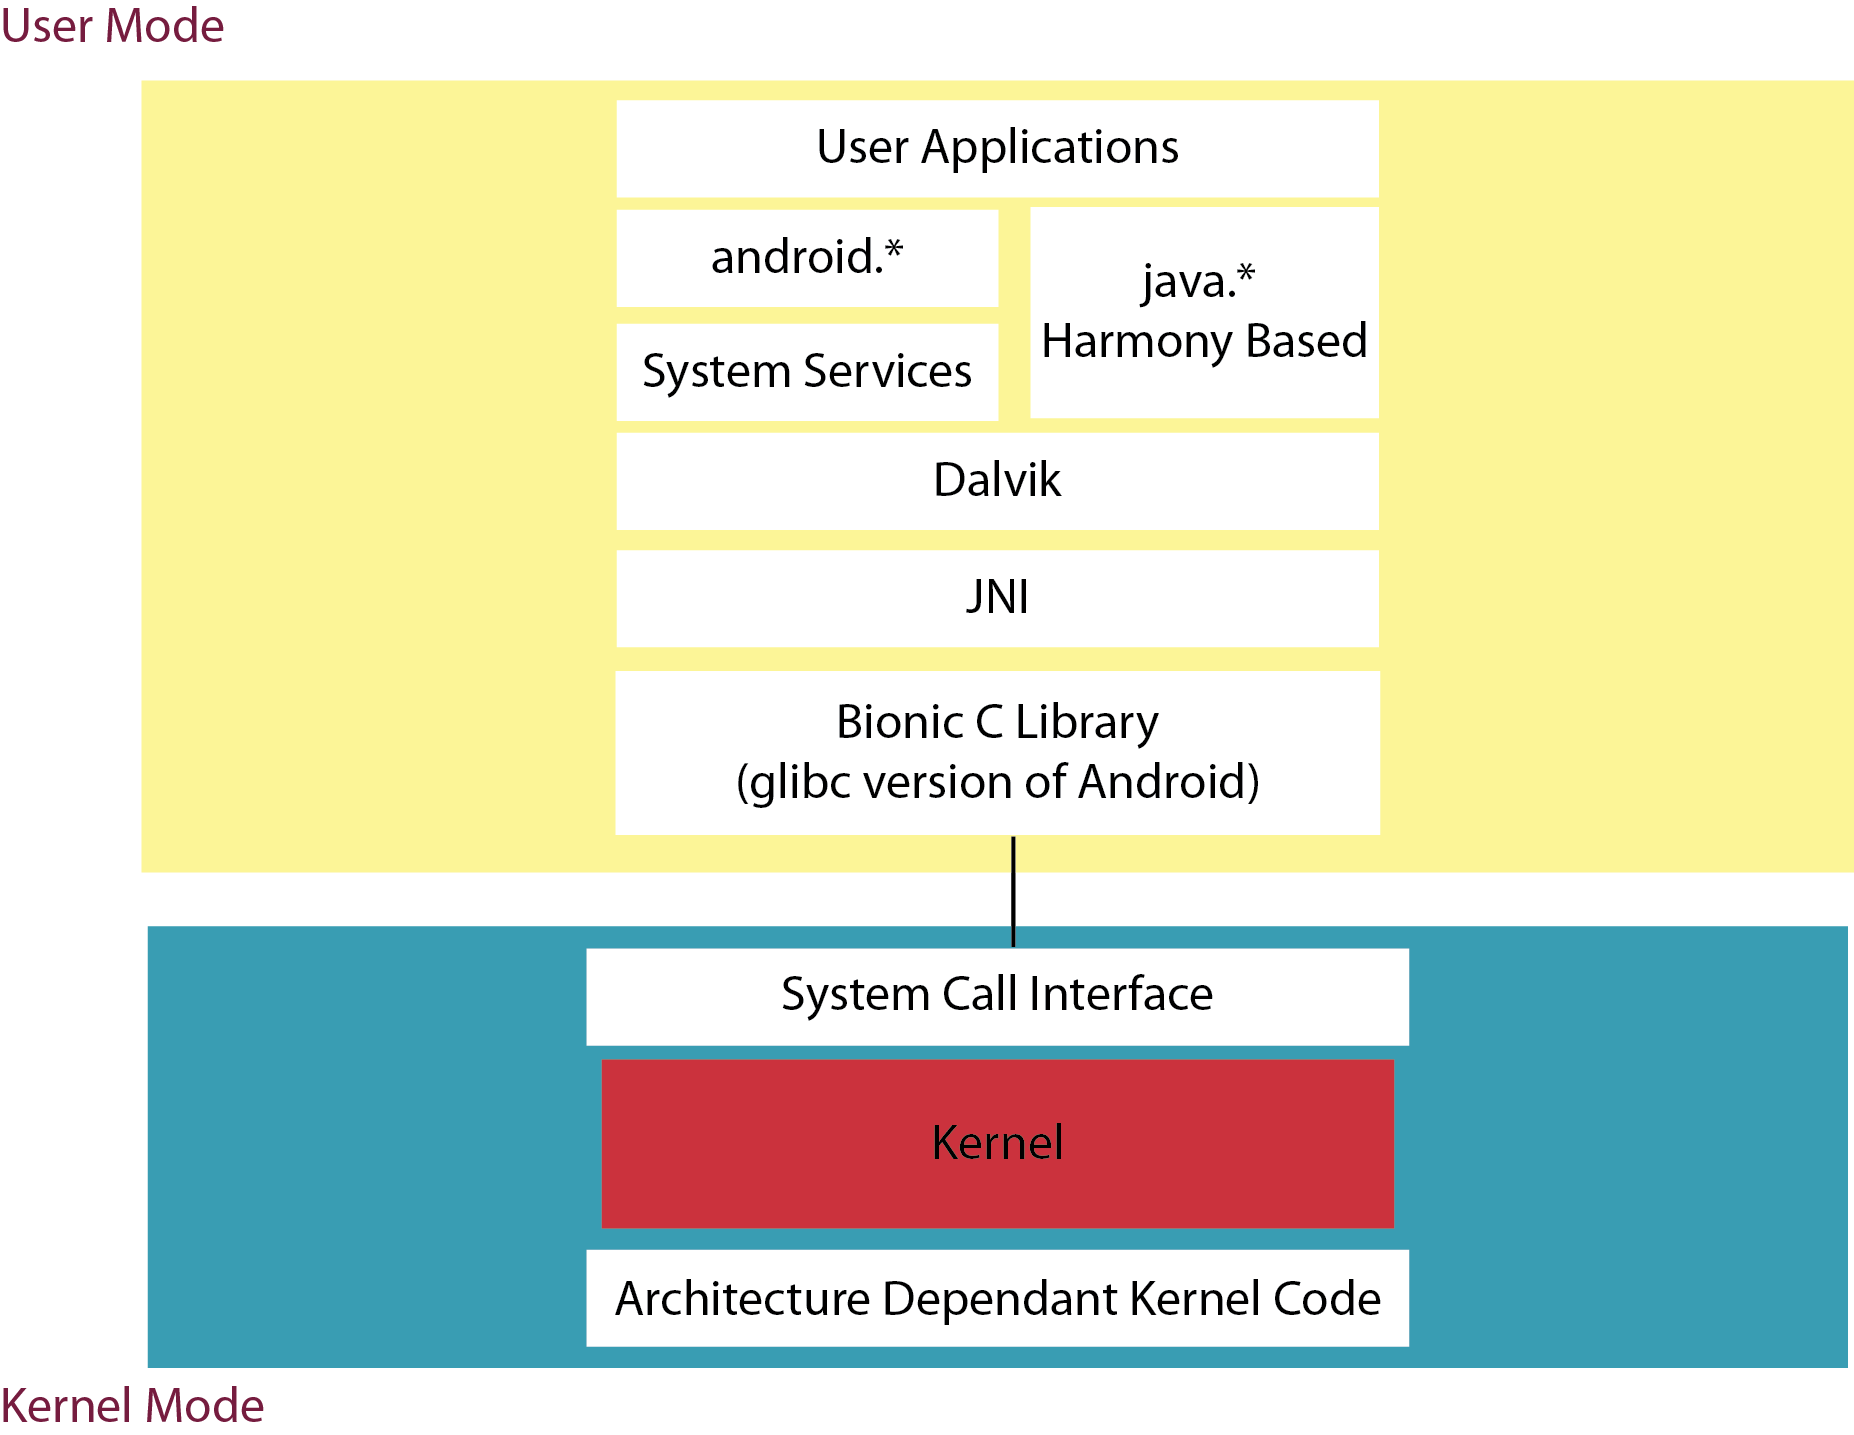
\includegraphics[width=\linewidth]{android-arch}
  \caption{Diagrama del kernel de Android}
  \label{fig:android-kernel}
\end{figure}


Como puede observarse. Android utiliza como base el kernel de linux y usa un
stack de la tecnología java de oracle como API e interfaz para los
desarrolladores. La maquina virtual java (JVM) funciona como un segundo kernel
que funciona encima de otro kernel. La JVM usada por Google esta desarrollada
especialmente para Android y se llama Dalvik. La primera capa JNI es usada para
hacer interfaz entre la máquina virtual y las aplicaciones nativas en
linux. Cabe mencionar que la máquina virtual o JVM esta desarrollada por Google
y tiene pornombre . Esta JVM no es la misma quelp oa desarrollada por
Oracle. Además de la libreria estandar de Java, Jvm contiene una librería
específica para dispositivos android. Esa solución es parecida a la
implementada en Windows Phone 7, sin embargo windows phone permite desarrollar
aplicaciones nativas sin jacer uso extensivo de .NET mientras que en Android
esto no es el objetivo.

\subsubsection{Mac OS X y iOS} El desarrollo de Mac OS X tiene lugar en un
momento clave de la compañía Apple. La estructura se muestra en la figura
\ref{fig:macosx-kernel}.

\begin{figure}[H]
  \centering
  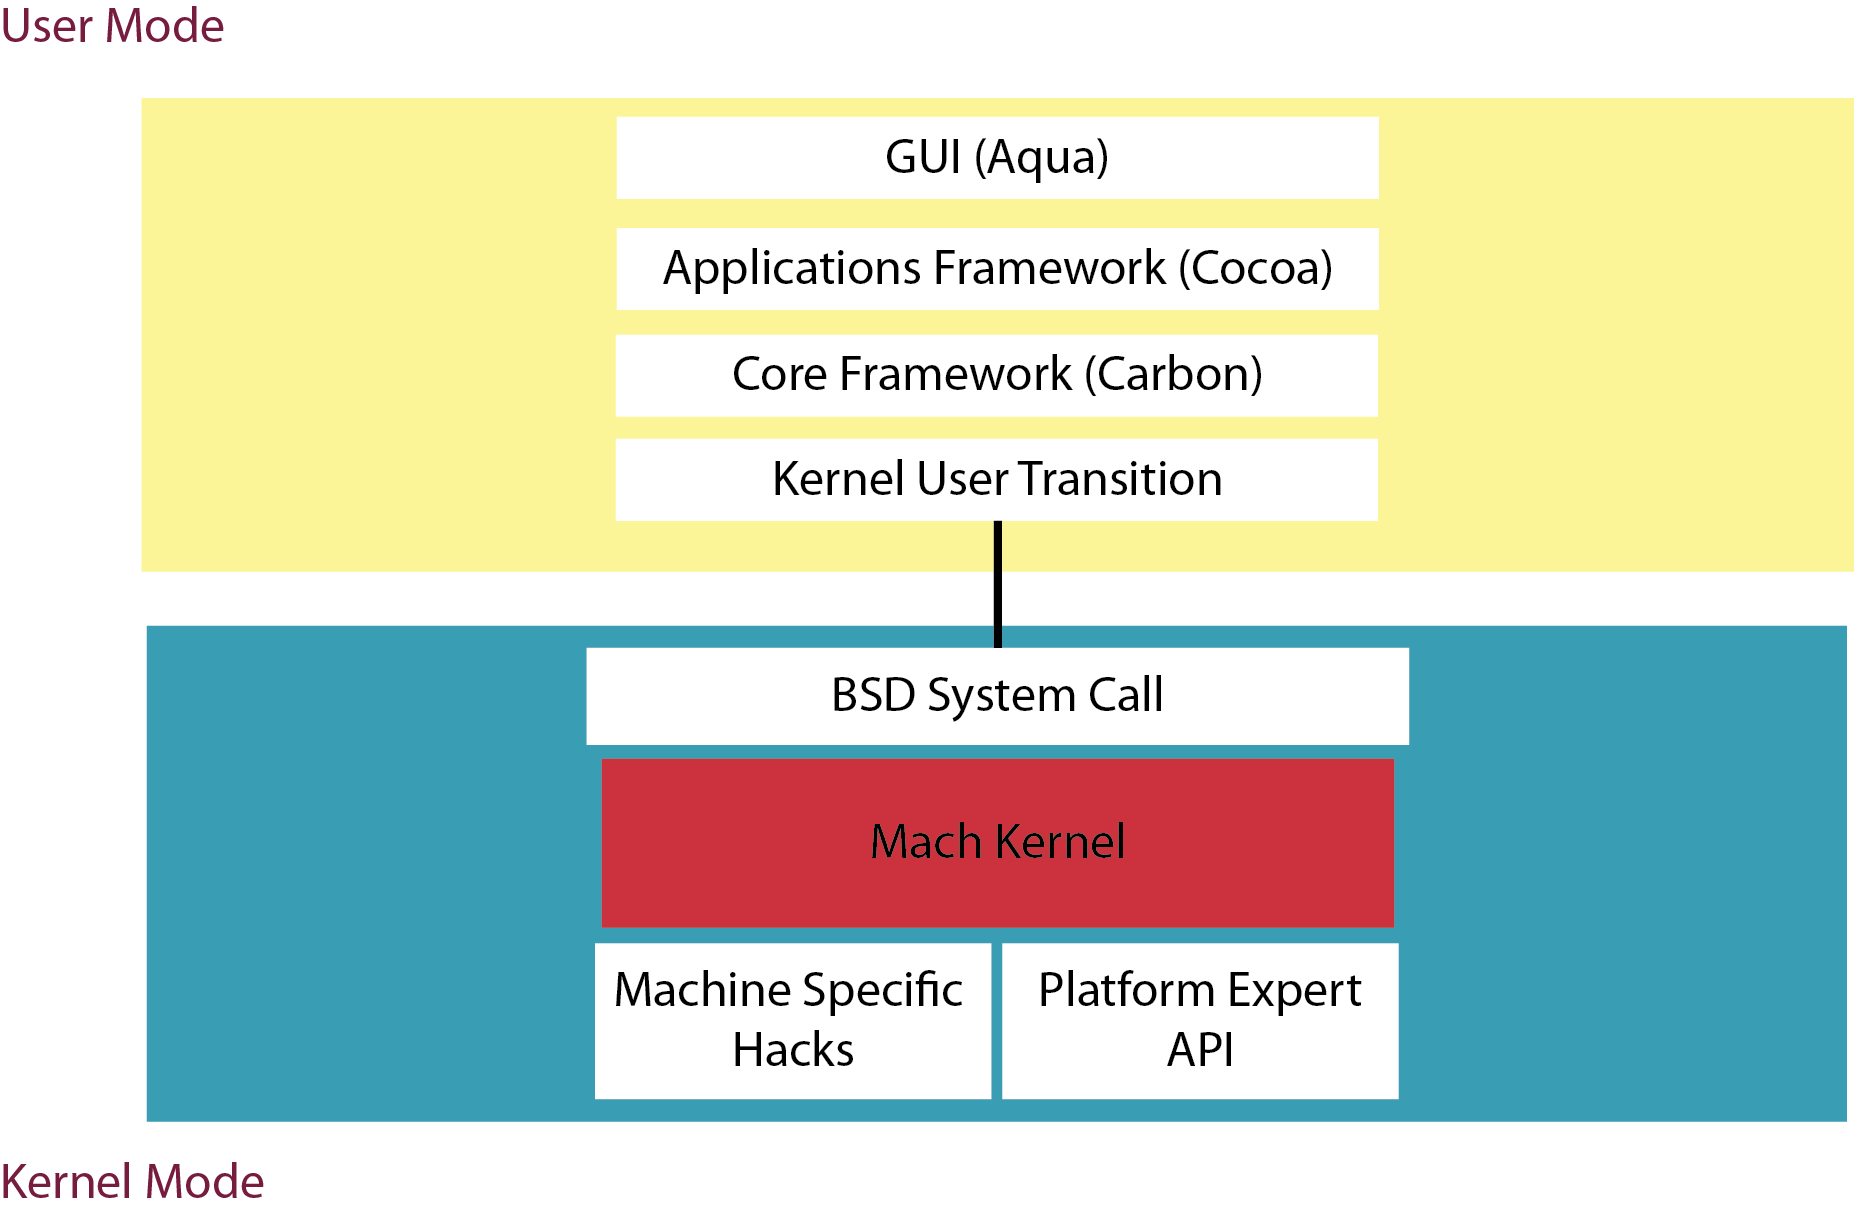
\includegraphics[width=\columnwidth]{osx-arch}
  \caption{Diagrama del kernel de Mac OS X}
  \label{fig:macosx-kernel}
\end{figure}

Hasta 1999, Apple había vendido computadoras con una arquitectura diferente a
la x86 desarrollada por IBM llamada PowerPC. Esto puede paracer confuso ya que
la PC fue desarrollada por IBM también, pero IBM solo licenció la arquitectura
x86. Actualmente las patentes x86 son otorgadas a Intel y AMD solamente a
diferencia de ARM que es open source. Regresando al tema de Apple, en 19 se
enfrentó a una crisis ante omniprecencia de la PC. Su antiguo CEO y fundador
Steve Jobs se encontraba separado de Apple y manejando la empresa NeXT. En esta
empresa se desarrollo un nuevo Unix usando la tecnología de microkernel
basándose en otro sostema operativo desarrolado en la academia llamado
Mach. Esta tecnología era novedosa y sin implementar en sistemas comerciales
hasta el momento. El sistema operativo tuvo por nombre NeXTStep. En una última
jugada, Apple adquiere NeXT junto con todas sus patentes para hacer frente a la
crisis, regresando a Steve Jobs como CEO. El previo sistema operativo de Apple,
Mac OS, es absorbido por NeXTStep y usando los conceptos de Mach crean el
kernel llamado Darwin, base del sistema operativo Mac OS X.  Como puede verse
en la figura \ref{fig:macosx-kernel}, Mac OS X es la fusión de conceptos de
Mach con otro sistema Unix llamado BSD. Aunque esto se ve en principio como una
solución pobre, el desarrollador no tiene que lidiar con esto ya que solo
necesita hacer uso del API escrito en Objetive C y Cocoa. Objetive C es un
subconjunto de C similar a C++ pero con una mayor orientación hacia el uso de
objetos. Cocoa es la interfaz o Framework que usa Objetive C para comunicarse
con el kernel darwin. Objetive C tambien fue desarrollado por NeXT antes de la
compra de Apple.

La versión móvil de Mac OS X es iOS. iOS utiliza la misma arquitectura que Mac
OS X. la única diferencia son las implementaciones de los servicios. Un ejemplo
es el sistema de archivos de iOS que esta orientado a memorias flash solamente
mientras que Mac OS X esta orientado a múltiples medios de
almacenamientos. Algo más evidente es el uso de diferentes interfaces de
usuario y sus APIs localizados en la capa superior. Mientras que Mac OS X
utiliza una libreria GUI llamada Aqua, iOS utiliza SpringBoard.

Como se puede notar, solo dos estándares están presentes en los diferentes
kernels: el propuesto por Microsoft y el estandar Unix. Por este motivo la
discusión en los siguientes capítulos se centrará en estos dos estándares y en
la JVM, la cual esta presente en todos los sistemas operativos y se puede
considerar como una implemetación mas de un sistema operativo. Sin embargo, se
mencionarán las diferencias pertinetes en los seis sistemas operativos de ser
necesario.

\subsection{Bootloader}
El proceso de arranque de la computadora consiste en la inicializacion de los
dispositivos y la carga del sistema operativo en memoria. Este proceso, aunque
estandar, no fué igual en los inicios de las computadoras.

En la época previa a las computadoras personales y a los dispositivos de
entrada actuales, el proceso de arranque variaba según las necesitades del
hardware y en su mayoría no contaban con un sistema operativo en disco. El
proceso de arranque que usaban iba de no contar con un sistema operativo y el
acceso a hardware era directo a memoria a traves de palancas y botones hasta
pequeñas secuencias de instrucciones programadas dentro de circuitos integrados
o sistemas basados en el uso de tarjetas perforadas. En la década de 1970,
diferentes compañias se dieron a la tarea de crear sistemas operativos que
ofrecieran las herramientas para explotar el hardware en el que fueran
instalados. En esta época era común ver computadoras funcionando usando
interpretes de lenguaje como BASIC o LISP donde el operador tenía que conocer
tanto el lenguaje como la arquitectura con la que estaba trabajando.

A mediados de la decada de los 70, IBM comenzo a implementar un plan comercial
conocido como ``chess project'' que más tarde sería el lanzamiento de la primera
computadora personal. Dentro de este plan se contemplaba que para poder
capturar el mercado se debería usar una arquitectura abierta y flexible además
de tener la facilidad de usar la computadora sin conocimientos profundos de su
funcionamiento. IBM se acerco a Bill Gates, entonces CEO de Microsoft, con la
petición de crear un sistema operativo que pudiera ser cargado desde discos
magnéticos, producto que IBM acababa de lanzar al mercado. Este sistema
operativo debería tener la capacidad de trabajar con diferente tipo de hardware
y poder presentar al usuario diferentes aplicaciones sin la necesidad de
conocer un lenguaje de programación. A su vez, la creación de un sistema
operativo portable abriría paso a un desarrollo más ágil de hardware. Microsoft
compra de la compañia Digital Research un prototipo de un sistema operativo
para discos, DOS por sus siglas en inglés. El sistema inicial, denominado QDOS
o \emph{Quick Dirty Operating System} fué modificado y preparado para su
distribución comercial. Dos sistemas fueron lanzados tanto por IBM, el PC-DOS,
como por microsoft, el MS-DOS. Más adelante otras compañias desarrollarían sus
propios sistemas, entre ellos cabe mencionar Apple y Novell. En respecto al
sistema Unix, este fué concebido previo a la IBM-PC pero luego fué adaptado
para ser compatible con este tipo de hardware.

Este tipo de sistemas, que son el defacto estandar de la industria para
computadoras personales o PCs compatibles con IBM, funcionan en conjunto con el
hardware de la computadora para poder inicializar el sistema. Para poder darle
la habilidad al hardware de arrancar con diferentes tipos de sistemas
operativos, el arranque se dividió en tres pasos: inicialización del hardware,
carga del sistema operativo e inicialización del sistema operativo. Existen
otros acercamientos como el caso del sistema operativo Linux que en el tercer
paso reinicializa el hardware. El primer y segundo paso son denominados
\emph{bootstrap}. La inicialización del hardware es llevada acabo por el Basic
Input-Output System o BIOS que es almacenado unidades ROM o Flash empotradas en
el hardware. Aunque el nuevo estandar, Extensible Firmware Interface o EFI,
esta reemplazando el antiguo BIOS, llamado ahora legacy BIOS, se estará usando
el término BIOS para ambos sistemas a menos que se mencione lo contrario en el
resto del curso.

El BIOS se encarga también de cargar en memoria el programa de carga o
bootloader de una dirección particular de las unidades de disco. En la
actualidad el BIOS puede cargar el bootloader dese múltiples sistemas de
almacenamiento. El bootloader se encarga de buscar y cargar el kernel del
sistema operativo en memoria.  Para poder escribir un bootloader se deben
considerar ciertas condiciones previas impuestas por el BIOS.

Primero, el BIOS busca el bootloader en el primer sector de la primera pista de
la primera cara del disco. Segundo, el BIOS requiere de una firma especial al
final del sector, los últimos dos bytes deben contener el valor \texttt{0xAA} y
\texttt{0x55}\footnote{La notación \texttt{Ox} hace referencia a un número
hexadecimal} respectivamente. Esta condición también introduce una restricción
de tamaño, el bootloader debe tener un tamaño de 512 bytes o un sector,
contando los dos últimos bytes de la firma. Una restricción también impuesta a
nivel de diseño es la retrocompatibilidad del BIOS con los sistemas operativos
de 16 bits, lo que restringe al cargador a operar en modo de 16 bits y
limitando el uso de memoria a $2^16$ direcciones de memoria, es decir, del
\texttt{0x0000} al \texttt{0xFFFF}. Una última característica de diseño es que
el BIOS cargará el bootloader en la dirección \texttt{0x7C00}. Por lo tanto,
todas las direcciones invocadas por el bootloader tienen como referencia la
dirección de carga. La razón de esta dirección en particular es debido a que
todos los dispositivos de I/O deben de ser asignados a una dirección de memoria
para su posterior invocación además de dejar espacio de sobra para cargar el
kernel. Esta desición fué tomada por los ingenieros de IBM al desarrollar la
IBM PC 5150, dejando el último kilobyte (1KB) de la memoria para el
bootloader. En ese entonces el mínimo para correr el PC-DOS era
32KB\footnote{\texttt{0x7C00} es el inicio del último KB en 32KB también es
representado como (\texttt{32KB} - \texttt{1KB})} .

En la tabla se muestra un bootloader que imprime la letra ``A''.

\lstinputlisting[style=customasm, caption=Un simple bootloader]{aboot.asm}

Las primeras dos líneas de código son directivas de compilador que indican la
operación en modo de 16 bits y que las direcciones usadas son relativas a la
posición inicial dada por el BIOS.

Ahora se presenta el problema del despliegue en pantalla. Debido a que no
tenemos el kernel cargado, no podemos hacer uso de ninguna librería. Para poder
imprimir en pantalla haremos uso de subrutinas de hardware llamadas
interrupciones. Una interrupción de hardware es invocada por la instruccion
\texttt{INT} seguida del número de la interrupción. La impresión en pantalla
toma cuatro argumentos: el caracter a imprimir en el registro \texttt{AL}, el
tipo de servicio en \texttt{BL}, colores del caracter en \texttt{BH} y. De
todas las propiedades tal vez la más confusa es el tipo de servicio almacenado
en \texttt{BL}. La interrupcion \texttt{0x10} que es la que vamos a invocar
proporciona múltiples servicios para la impresión en pantalla. El tipo de
servicio es indicado por un número de servicio definido en la arquitectura del
BIOS. Las siguientes dos lineas del código invocan a una subrutina preparada
para la impresión de un caracter en pantalla:

\lstinputlisting[style=customasm, linerange=5-6, numbers=none]{aboot.asm}

La primera linea almacena en \texttt{AL} el caracter a imprimir en código
ASCIII, 67 para la letra A. La segunda línea llama a la subrutina de impresión.

\lstinputlisting[style=customasm, linerange=10-17, numbers=none]{aboot.asm}

El cuerpo de la subrutina prepara los datos para llamar a la interrupción
necesaria. \texttt{AH} almacena el tipo de servicio para impresión en pantalla
\texttt{0xE0}. \texttt{BL} contiene la página en la que se encuentra la zona de
memoria del monitor. Por el momento este concepto se dejará para temas más
adelante, no se preocupe en entenderlo. El último dato que describe el apecto
del caracter a imprimir se coloca en \texttt{BH}. Se eligió color gris sobre
fondo negro. Por último se llama a la interrupcion \texttt{0x10}\footnote{en
lenguaje ensamblador los numeros hexadecimales se denotan por $n$ dígitos
seguidos de la letra H}.

Por último se cicla a la computadora en un ciclo infinito con la instrucción:

\lstinputlisting[style=customasm, linerange=7-7, numbers=none]{aboot.asm}

Las siguientes instrucciones requiere un poco mas de explicación:

\lstinputlisting[style=customasm, linerange=19-20, numbers=none]{aboot.asm}

Note que nuestro programa debería de hacer un ciclo infinito en la última
instrucción descrita. Por lo tanto estas dos lineas no se alcanzarían en un
flujo de ejecución. Sin embargo estas dos instrucciónes son directivas de
compilador. La primera nos sirve para rellenar nuestro código binario
resultante para que ocupe 510 Bytes. El símbolo \texttt{\$\$} apunta a la
dirección inicial de nuestro programa. Por lo tanto calculamos el espacio total
que ocupa nuestras instrucciones contando la actual y el total se lo restamos a
510. Esto nos da la cantidad necesaria de \texttt{0} colocados en el código
máquina al ser compilado. La siguiente instrucción coloca en el código máquina
resultante la firma del bootloader en los dos últimos bytes.

Para crar el código máquina necesitamos un compilador de ensamblador, en
windows, linux y osx podemos usar NASM\footnote{\url{http://www.nasm.us}}. Para
compilarlo en NASM se utilíza la siguiente instrucción


\begin{lstlisting}[style=custombash, caption=Compilando el bootloader con NASM]
  nasm aboot.asm -f bin -o boot.bin
\end{lstlisting}

con esta instrucción le pedimos la compilador una salida binaria sin encabezado
de nuestro programa. El tema de encabezados se vera más adelante. El último
paso es colocar el programa obtenido en el MBR. Unix tiene por defecto la
instrucción de consola \texttt{dd}. En esta ocasión lo colocaremos en una
unidad virtual para ser cargada con \emph{Virtual Box} \footnote{\url{http://www.virtualbox.org}}.
La lista de comandos siguientes en linux sirven para crear una imagen virtual
de un floppy, crear un directorio donde montar el floppy, montar el floppy,
escribir nuestro bootloader y desmontar la unidad \footnote{Las instrucciones
  se tomaron en cuenta en una instalación de linux sobre una máquina virtual
  como se muestra en los videos del curso con liga \url{}}. 

\begin{lstlisting}[style=custombash, caption=Preparando un floppy virtual]
  mkfs.dos -C floppy.img 1440
  sudo mkdir /mnt/vfloppy
  sudo mount -o loop floppy.img /mnt/vfloppy 
  sudo dd if=boot.bin bs=512 of=/mnt/vfloppy
\end{lstlisting}

Por último colocamos el floppy en la máquina virtual e iniciamos la máquina
virtual. Despues del self test de la maquina virtual podemos ver como la A aparece en
pantalla y la máquina virtual queda suspendida en un ciclo infinito.
% \end{document}                  

%%% Local Variables: 
%%% mode: latex
%%% TeX-master: "index"
%%% End: 

\end{document}